\section{Die Hardware}

Das Ziel bei der Hardwarewahl ist es möglichst günstige und weit 
verbreitete Komponenten zu wählen. So kann der Synthesizer
leicht nachgebaut werden.

\subsection{ESP32-S3}


\begin{figure}[H]
    \begin{center}
        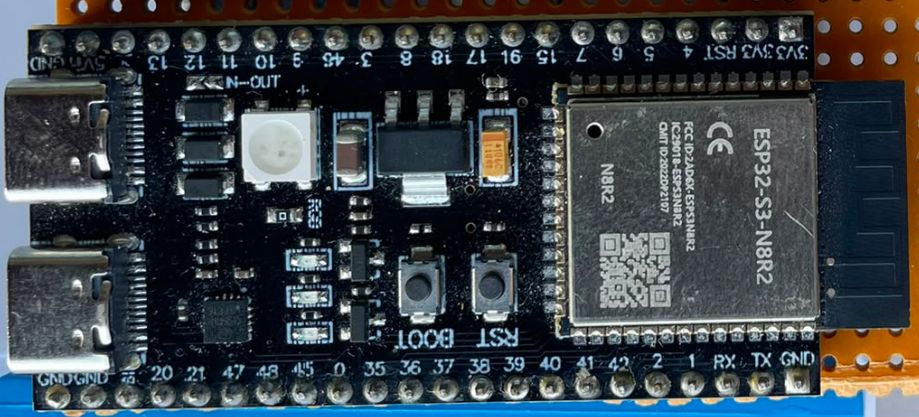
\includegraphics[width=8cm]{fig/components/ESP32S3.png}
        \caption{ESP32-S3 Entwicklingsboard.}%
        \label{fig:ESP32S3}
    \end{center}
\end{figure}

Neben Arduino-boards \cite{arduino} sind ESP32-boards von Espressif Systems
\cite{espressif} die bekanntesten
Microkontrollerboards. Außerdem sind sie für unter 10 € günstig erhältlich.

Ein ESP32 ist ein Microkontroller mit einer 
32-Bit-Dual-Core-CPU, die mit 240MHz betrieben werden kann.
Bei einer Abtastrate von 44100 lässt sich jeder Wert im Durchschnitt
mit ca. 5000 Taktzyklen bearbeiten und es steht ein weiterer Kern für
andere Funktionen zur Verfügung.
\begin{center}
$240MHz / 44100Hz = 5442$
\end{center}
Der ESP32-S3 wurde anderen ESP32 Mikrokontrollern vorgezogen, da er
spezielle Hardware besitzt, um DSP-Operationen zu beschleunigen. Zum 
Beispiel hat er spezielle Register für 128-Bit-Operationen.

Der ESP32 hat dazu den Vorteil gegenüber anderen Microcontrollern, dass
er viel GPIO pins und viele Perepherieschnittstellen hat. Wichtig für dieses
Projekt sind vorallem I2C, I2S.

\subsection{MAX98357A-I2S-DAC}

\begin{figure}[H]
    \begin{subfigure}{0.48\textwidth}
    \begin{center}
        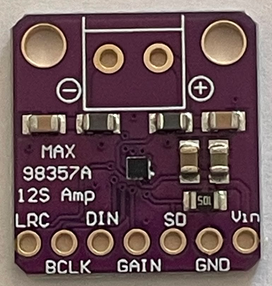
\includegraphics[width=4cm]{fig/components/dac_front.png}
    \end{center}
    \end{subfigure}
    \hfill
    \begin{subfigure}{0.48\textwidth}
    \begin{center}
        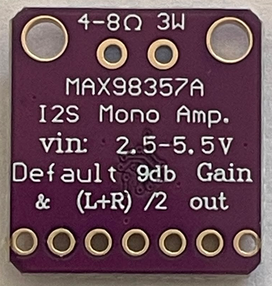
\includegraphics[width=4cm]{fig/components/dac_back.png}
    \end{center}
    \end{subfigure}
\caption{MAX98357A-I2S-DAC}
\label{fig:DAC}
\end{figure}

Ein MAX98357A-DAC (Digital-to-Analog Converter) \cite{MAX983572026Datasheet}
wandelt das digitale Signal in analoges Signal um und verstärkt es so, dass es
direkt an einen passenden Lautsprecher weitergeleitet werden kann.
Der MAX98357A kann Abtatsraten von 8kHz, 16kHz, 32kHz, 44.1kHz,
48kHz, 88.2kHz oder 96kHz und eine Auflösung von 
16, 24 oder 32 Bit
verarbeiten \cite{MAX983572026Datasheet}[Digital Audio Interface Modes].

Das analoge Signal wird von dem DAC zu einer 3,5mm-Klinkenbuchse geleitet. 
So kann leicht ein Lautsprecher angeschlossen werden. Klingenstecher sind 
unterteilt in mehrere segmente und haben in der Regel die Masseverbindung 
an dem ring, der am nächsten am kabel ist. Deshalb wird der vorderste Pin 
der Buchse mit dem negativen Ausgang des DACs verbunden. Da der MAX98357A 
ein Monosignal (nur ein Signal und nicht rechts und links) sendet, werden 
die beiden anderen Pins der Buchse mit dem Positiven Ausgang verbunden.
 
TODO Quelle zu Klinke

\begin{figure}[H]
    \begin{subfigure}{0.48\textwidth}
    \begin{center}
        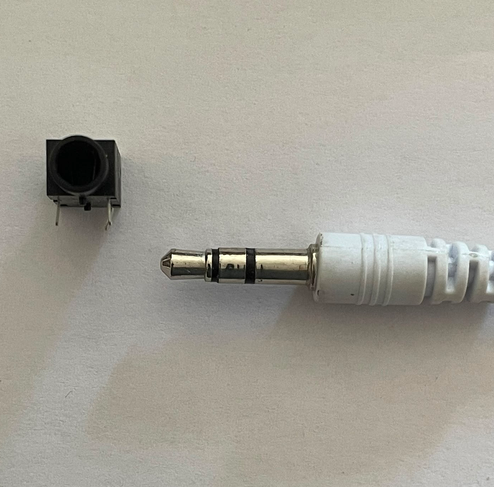
\includegraphics[width=4cm]{fig/components/aux_front.png}
    \end{center}
    \end{subfigure}
    \hfill
    \begin{subfigure}{0.48\textwidth}
    \begin{center}
        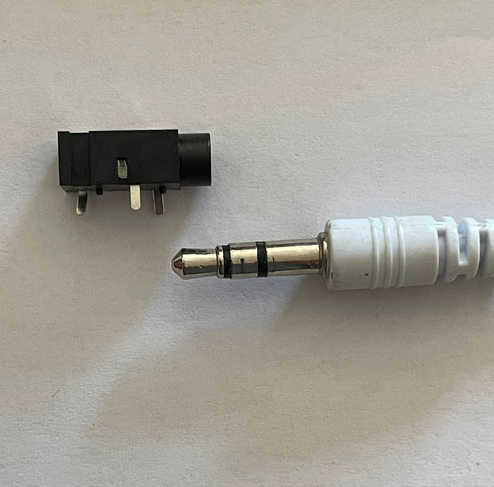
\includegraphics[width=4cm]{fig/components/aux_side.png}
    \end{center}
    \end{subfigure}
\caption{Klinkenbuchse und Stecker}
\label{fig:AUX}
\end{figure}

\subsection{Taster und Drehgeber}

Als Nutzereingabe werden Taster und ein Drehgeber verwendet.

\begin{figure}[H]
    \begin{subfigure}{0.48\textwidth}
    \begin{center}
        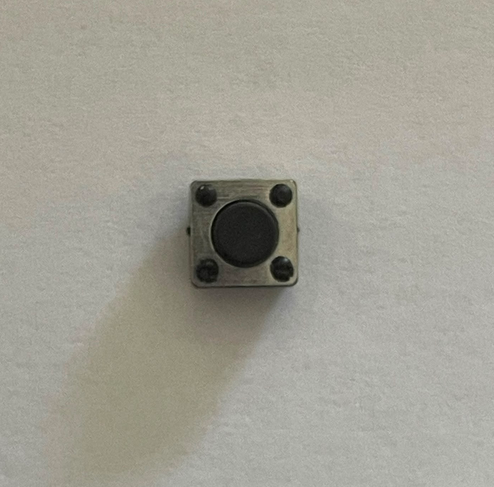
\includegraphics[width=4cm]{fig/components/button_top.png}
    \end{center}
    \end{subfigure}
    \hfill
    \begin{subfigure}{0.48\textwidth}
    \begin{center}
        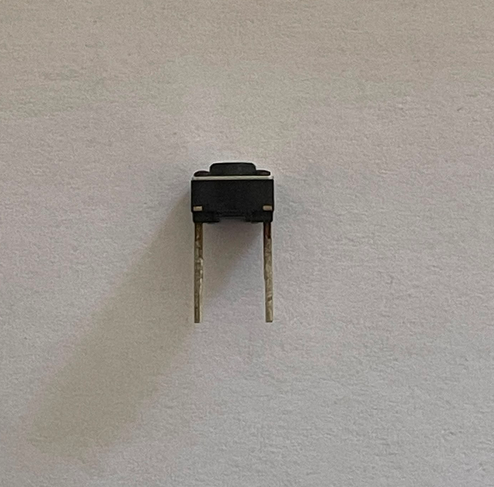
\includegraphics[width=4cm]{fig/components/button_side.png}
    \end{center}
    \end{subfigure}
\caption{Einfacher Taster}
\label{fig:Taster}
\end{figure}


Ein Taster lässt nur Strom durch, wenn er gedrückt wird. Der ESP32-S3 
kann an den meisten GPIO-Pins (General Purpose Input/Output)erkennen,
ob ein High- oder Low-Pegel anliegt. Schaltet man den einen Taster und 
eine Resistor (z.B. 10k) in Reihe ,also nacheinander, zwischen der Masse
und einen GPIOpin, so wird dieser auf LOW gesetzt, wenn der Taster gedrückt
wird. Ist der Pullup an diesem Pin aktiviert, wird der Pin HIGH gesetzt, 
wenn nichts an dem Pin anliegt. Also, auch wenn der Taster nicht gedrückt 
wird.

\begin{figure}[H]
    \begin{subfigure}{0.48\textwidth}
    \begin{center}
        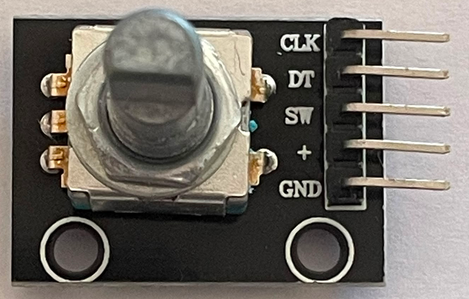
\includegraphics[width=4cm]{fig/components/encoder_top.png}
    \end{center}
    \end{subfigure}
    \hfill
    \begin{subfigure}{0.48\textwidth}
    \begin{center}
        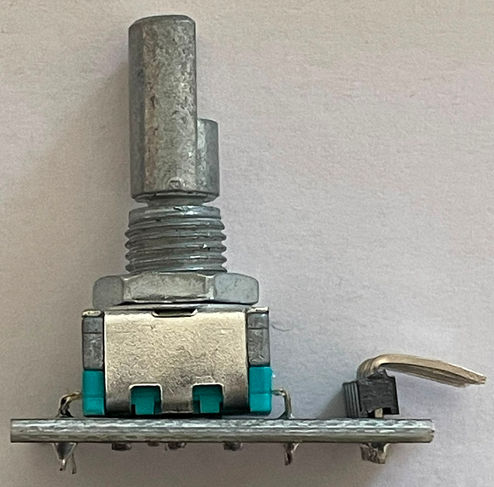
\includegraphics[width=4cm]{fig/components/encoder_side.png}
    \end{center}
    \end{subfigure}
\caption{Drehgeber}
\label{fig:Drehgeber}
\end{figure}

Ein incrementeller Drehregler kann mithilfe von zwei versetzten Impulsen, 
welche auf dem DT und CLK Pin des Encoders gesendet werden, angeben in welche
Richtung er gedreht wird. Diese Pins müssen mit GPIO-Pins des ESP32-S3 
verbunden werden. Zusätzlich kann der Encoder als Taster genutzt werden,
in dem man den Schaft drückt.

Mit 10 Tastern und einem Drehgeber ist es möglich,
während der Laufzeit verschiedene Variablen zu bearbeiten.
Die genaue Finktion der Taster wird in Kapitel 7 beschrieben.

\subsection{OLED-BildSchirm}

\begin{figure}[H]
    \begin{subfigure}{0.48\textwidth}
    \begin{center}
        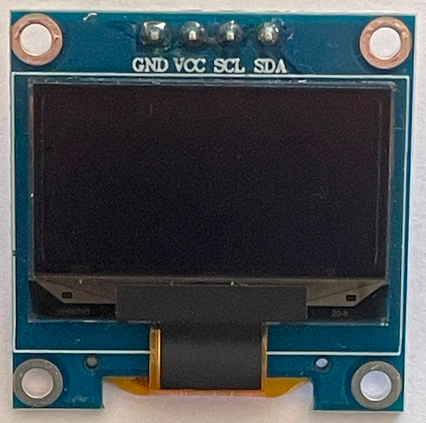
\includegraphics[width=4cm]{fig/components/screen_front.png}
    \end{center}
    \end{subfigure}
    \hfill
    \begin{subfigure}{0.48\textwidth}
    \begin{center}
        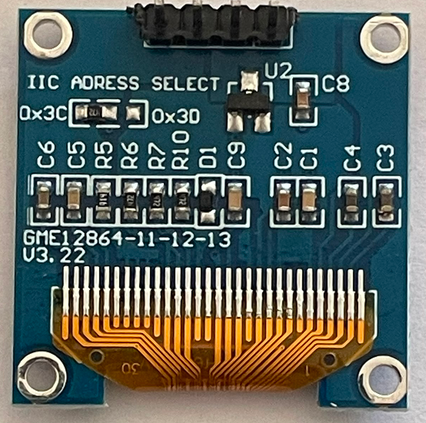
\includegraphics[width=4cm]{fig/components/screen_back.png}
    \end{center}
    \end{subfigure}
\caption{OLED-Bildschirm}
\label{fig:OLED-Bildschirm}
\end{figure}

Ein OLED-Bildschirm wird genutzt, um dem Nutzer anzuzeigen, welche
Variable geändert wird. Die Verbindung zum ESP32 passiert über das
I2C-Protokoll.

\subsection{Pinbelegung und Löten}

Nun müssen alles Komponenten mit dem ESP32S3 verbunden werden.
Der ESP32S3 hat intern eine GPIO Matrix\cite{esp32S3gpio}, welche es ermöglicht fast
jeden internen Perepheriecontroller mit fast jedem Pin zu verbinden.

Zusätzlich zu den oben aufgezählten Komponenten wurden ein SD-Karten
slot über die SPI-Schnittstelle als mögliche Erweiterung verbunden.

Die Wahl der Pins ist für I2S, I2C und GPIO fast immer frei wählbar.
Es ist zwar möglich die folgenden Ausnahmen zu benutzen, aber nicht empfehlen.
\begin{itemize}
    \item Pins 19 und 20 sind mit dem JTAG-Debugger verbunden.
    \item Pins 44 und 48 sind mit den eingebauten LEDs verbunden.
    \item Pins 0, 3, 45 und 46 sind Strappingpins. Das sind Pins, die das Bootverhalten
            ändern können jenachdem, ob an ihnen, während des Bootvorgangs, ein 
            High- oder Low-Pegel anliegt.
    \item Pins 33-37 sind verbunden mit dem SPI-flash and PSRAM auf dem 
    Entwicklingsboard.
\end{itemize}

Mit diesen Einschränkungen wurde die Pinbelegung aus Anhang A gewählt.
Anschließend wurde alles auf eine Lochplatine gelötet.

\begin{figure}[H]
    \begin{subfigure}{0.48\textwidth}
    \begin{center}
        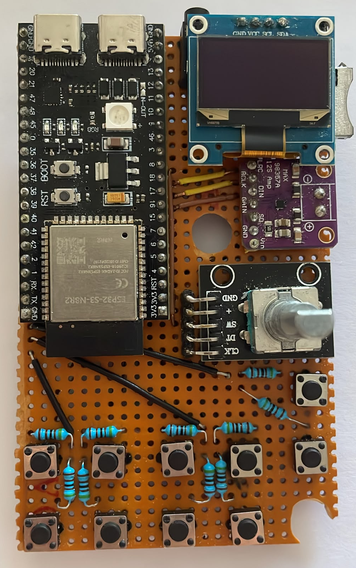
\includegraphics[width=6cm]{fig/case/platine_front.png}
    \end{center}
    \end{subfigure}
    \hfill
    \begin{subfigure}{0.48\textwidth}
    \begin{center}
        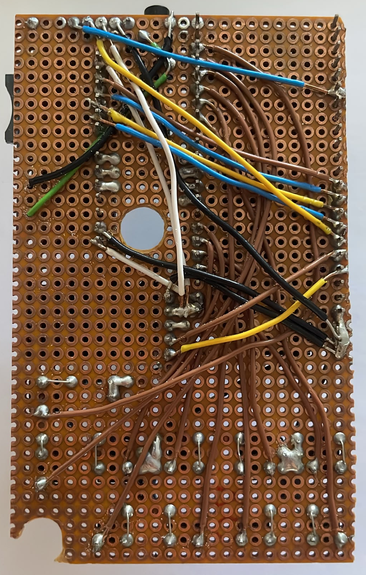
\includegraphics[width=6cm]{fig/case/platine_back.png}
    \end{center}
    \end{subfigure}
\caption{Lochplatine mit angelöteten Komponenten}
\label{fig:platine}
\end{figure}


\subsection{Design und Drucken einer Hülle}
Als Abschluss der Hardware wurde die folgende Hülle 3D-gedruckt.

\begin{figure}[H]
    \begin{subfigure}{0.48\textwidth}
    \begin{center}
        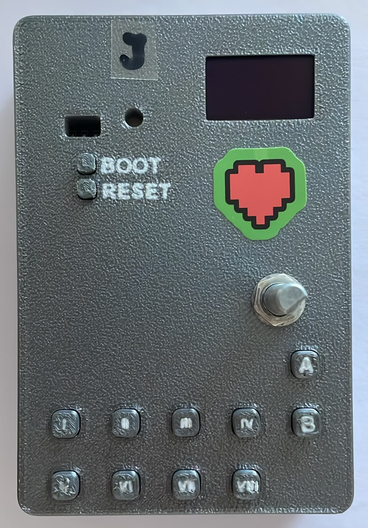
\includegraphics[width=6cm]{fig/case/assembled_front.png}
    \end{center}
    \end{subfigure}
    \hfill
    \begin{subfigure}{0.48\textwidth}
    \begin{center}
        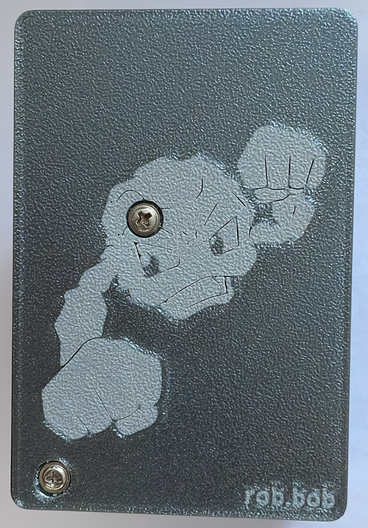
\includegraphics[width=6cm]{fig/case/assembled_back.png}
    \end{center}
    \end{subfigure}
\caption{Eine Hülle für die Platine}
\label{fig:hülle_außen}
\end{figure}

Zum Erstellen des 3D-Objektes wurde Fusion360\cite{fusion360} verwendet.
In Fusion360 ist es möglich ein Bild als Referenz zu laden. 
Das hat sich als schneller und genauer herausgestellt, als Maße von der 
Platine zu nehmen.

Zunächst wurde ein dünner Prototyp der Vorderseite gedruckt, da diese die 
meisten Öffnungen hat. Nach ein paar kleinen Anpassungen wurden die 
Seitenwände mit einer kleinen Einkerbung am Ende erstellt. Nach Maßen
wurden Löcher für die USB-, Aux- und SD-Karten-Anschlüsse hinzugefügt.

TODO 2 Figures

\begin{figure}[H]
    \begin{subfigure}{0.36\textwidth}
        \begin{center}
            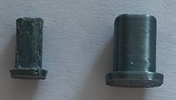
\includegraphics[height=2.5cm]{fig/case/buttons.png}
        \end{center}
        \caption{Knöpfe von der Seite}
    \end{subfigure}
    \hfill
    \begin{subfigure}{0.60\textwidth}
        \begin{center}
            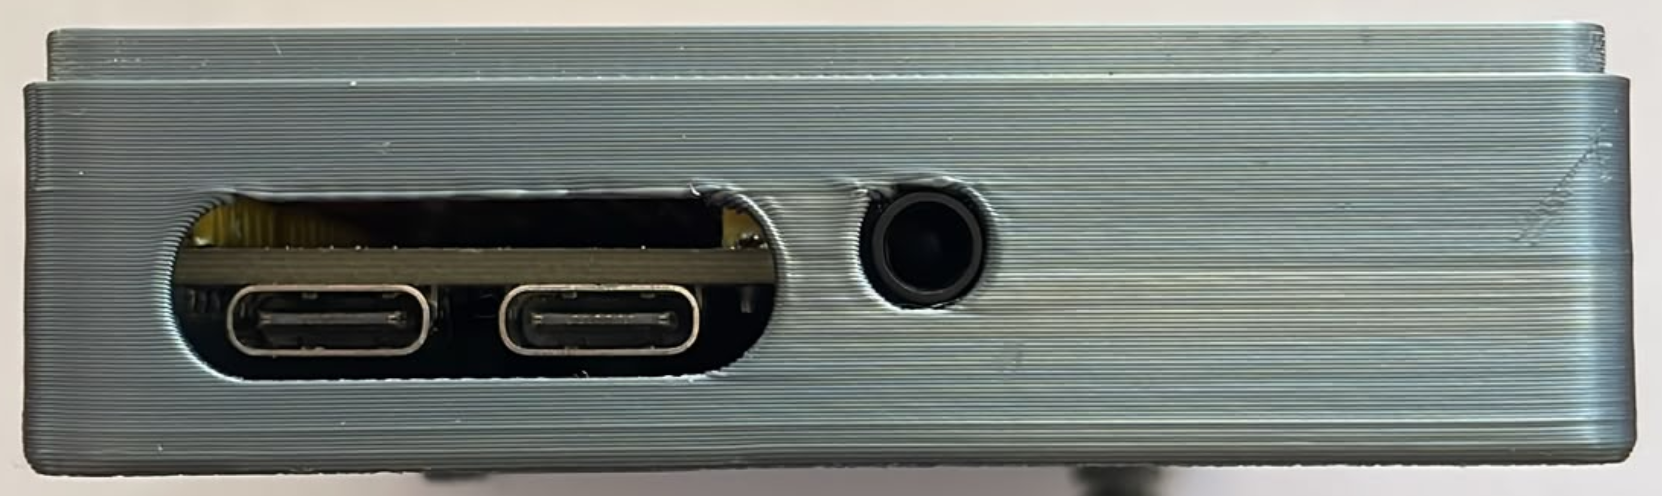
\includegraphics[height=2.5cm]{fig/case/case_top.png}
        \end{center}
        \caption{Oberseite Vorderseite der Hülle}
    \end{subfigure}
\label{fig:hülle_oben}
\end{figure}

In die Löcher für die Taster kommen kleine Knöpfe, die genau in die 
Löcher passen, aber unten etwas breiter sind damit sie nicht hinausfallen.
Für den Boot- und Resetknopf auf dem ESP32-S3 gibt es Auch jeweils einen Knopf.
Die sind allerdings kleiner. 

Auf der Platine gibt es 2 größere freie Flächen. Diese wurden genutzt 
um 2 Löcher zu boren, durch die 2 Säulen laufen. Die Mittelpunkte der Löcher liegen genau auf den kleinen Löchern der 
Platine, so wird der Boher fixiert und in Fusion360 kann der Mittelpunkte
der Säulen leicht ermittelt werden. 

TODO Bild von einschmelzgewinde

In die Spitze der Säulen wurden Einschmelzgewinde eingeschmolzen. Dazu wurde 
in der Säule ein Loch, das etwas kleiner ist als der Außendurchmesser des
Gewindes, gelassen. Anschließend setzt man das Gewinde auf das Loch und 
drückt es herunter, indem man einen heißen Lötkolben in das gewinde drückt.
Dadurch heizt sich das Gewinde auf und schmiltzt das Plastik.

Die Säulen halten auch die platine am richtigen platz.


\begin{figure}[H]
    \begin{subfigure}{0.48\textwidth}
    \begin{center}
        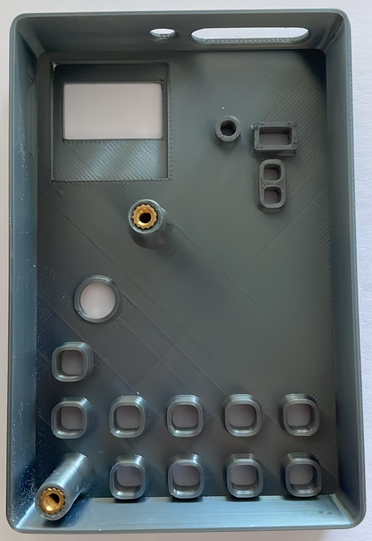
\includegraphics[width=6cm]{fig/case/front_case_inside.png}
    \end{center}
    \end{subfigure}
    \hfill
    \begin{subfigure}{0.48\textwidth}
    \begin{center}
        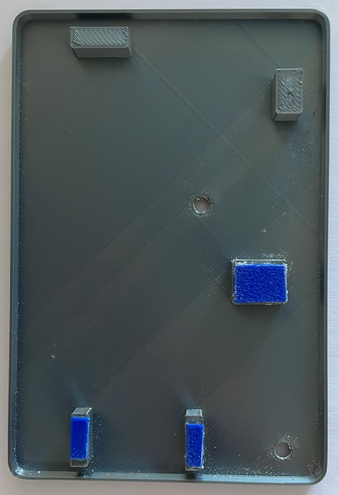
\includegraphics[width=6cm]{fig/case/back_case_inside.png}
    \end{center}
    \end{subfigure}
\caption{Innenseite der Hülle}
\label{fig:hülle_innen}
\end{figure}

Legt man die Platine in die Oberseite der Hülle, so liegen die Taster auf den
Knöpfen auf. Damit die Platine beim Drücken der Knöpfe nicht nach hinten
gedrückt wird, wurde auf die Innenseite der Rückwand Blöcke als 
Abstandshalter gedruckt. Einige der Blöcke wurden nach dem Drucken der 
RÜckseite durch Aufkleben von blauen platten erhöht.